% answers.tex —— 2008 年·普通高等学校招生考试·辽宁卷·理科 · 参考答案与详细解析片段
% 由 tools/generate_projects.py 依来源总账自 2008/2008_数学真题_辽宁理_试题.md + 2008/2008_数学真题_辽宁理_解析正文.md + 2008/2008_数学真题_辽宁理_答案要点.md 生成，勿手改（改源 MD 后重跑）


\begin{gktip}
固定候选 PDF 仅含题面，无答案、解析和评分标准；以下为非官方编者独立推导。
\end{gktip}

\begin{answer}
\gksolhead{1}{}

\textbf{题目}：

已知集合 $M=\left\{x\mid \dfrac{x+3}{x-1}<0\right\}$，$N=\{x\mid x\leqslant-3\}$，则集合 $\{x\mid x\geqslant1\}=$（　）

（A）$M\cap N$

（B）$M\cup N$

（C）$\complement_{\mathbf R}(M\cap N)$

（D）$\complement_{\mathbf R}(M\cup N)$

\Needspace{4\baselineskip}
\textbf{解析}

$M=(-3,1)$，$N=(-\infty,-3]$，故 $M\cup N=(-\infty,1)$，$\complement_{\mathbf R}(M\cup N)=[1,+\infty)$。

\gkanswer{答案：D。}

\end{answer}
\begin{answer}
\gksolhead{2}{}

\textbf{题目}：

$\lim\limits_{n\to\infty}\dfrac{1+3+5+\cdots+(2n-1)}{n(2n+1)}=$（　）

（A）$\dfrac14$

（B）$\dfrac12$

（C）$1$

（D）$2$

\Needspace{4\baselineskip}
\textbf{解析}

分子为 $n^2$，故极限为 $\lim\dfrac{n^2}{n(2n+1)}=\dfrac12$。

\gkanswer{答案：B。}

\end{answer}
\begin{answer}
\gksolhead{3}{}

\textbf{题目}：

圆 $x^2+y^2=1$ 与直线 $y=kx+2$ 没有公共点的充要条件是（　）

（A）$k\in(-\sqrt2,\sqrt2)$

（B）$k\in(-\infty,-\sqrt2)\cup(\sqrt2,+\infty)$

（C）$k\in(-\sqrt3,\sqrt3)$

（D）$k\in(-\infty,-\sqrt3)\cup(\sqrt3,+\infty)$

\Needspace{4\baselineskip}
\textbf{解析}

圆心到 $kx-y+2=0$ 的距离 $\dfrac2{\sqrt{k^2+1}}>1$，即 $k^2<3$。

\gkanswer{答案：C。}

\end{answer}
\begin{answer}
\gksolhead{4}{}

\textbf{题目}：

复数 $\dfrac1{-2+\mathrm i}+\dfrac1{1-2\mathrm i}$ 的虚部是（　）

（A）$\dfrac15\mathrm i$

（B）$\dfrac15$

（C）$-\dfrac15\mathrm i$

（D）$-\dfrac15$

\Needspace{4\baselineskip}
\textbf{解析}

$\dfrac1{-2+\mathrm i}=\dfrac{-2-\mathrm i}5$，$\dfrac1{1-2\mathrm i}=\dfrac{1+2\mathrm i}5$，和为 $\dfrac{-1+\mathrm i}5$，虚部为 $\dfrac15$。

\gkanswer{答案：B。}

\end{answer}
\begin{answer}
\gksolhead{5}{}

\textbf{题目}：

已知 $O$，$A$，$B$ 是平面上的三个点，直线 $AB$ 上有一点 $C$，满足 $2\overrightarrow{AC}+\overrightarrow{CB}=\boldsymbol 0$，则 $\overrightarrow{OC}=$（　）

（A）$2\overrightarrow{OA}-\overrightarrow{OB}$

（B）$-\overrightarrow{OA}+2\overrightarrow{OB}$

（C）$\dfrac23\overrightarrow{OA}-\dfrac13\overrightarrow{OB}$

（D）$-\dfrac13\overrightarrow{OA}+\dfrac23\overrightarrow{OB}$

\Needspace{4\baselineskip}
\textbf{解析}

由 $2\overrightarrow{AC}+\overrightarrow{CB}=\boldsymbol 0$ 得 $2(C-A)+(B-C)=0$，即 $C=2A-B$，故 $\overrightarrow{OC}=2\overrightarrow{OA}-\overrightarrow{OB}$。

\gkanswer{答案：A。}

\end{answer}
\begin{answer}
\gksolhead{6}{}

\textbf{题目}：

设 $P$ 为曲线 $C:y=x^2+2x+3$ 上的点，且曲线 $C$ 在点 $P$ 处切线倾斜角的取值范围是 $\left[0,\dfrac{\pi}{4}\right]$，则点 $P$ 横坐标的取值范围是（　）

（A）$\left[-1,-\dfrac12\right]$

（B）$[-1,0]$

（C）$[0,1]$

（D）$\left[\dfrac12,1\right]$

\Needspace{4\baselineskip}
\textbf{解析}

$y'=2x+2$，由 $\tan\theta\in[0,1]$ 得 $-1\leqslant x\leqslant-\dfrac12$。

\gkanswer{答案：A。}

\end{answer}
\begin{answer}
\gksolhead{7}{}

\textbf{题目}：

$4$ 张卡片上分别写有数字 $1$，$2$，$3$，$4$，从这 $4$ 张卡片中随机抽取 $2$ 张，则取出的 $2$ 张卡片上的数字之和为奇数的概率为（　）

（A）$\dfrac13$

（B）$\dfrac12$

（C）$\dfrac23$

（D）$\dfrac34$

\Needspace{4\baselineskip}
\textbf{解析}

一奇一偶：$\dfrac{2\times2}{\mathrm C_4^2}=\dfrac23$。

\gkanswer{答案：C。}

\end{answer}
\begin{answer}
\gksolhead{8}{}

\textbf{题目}：

将函数 $y=2^x+1$ 的图象按向量 $\boldsymbol a$ 平移得到函数 $y=2^{x+1}$ 的图象，则（　）

（A）$\boldsymbol a=(-1,-1)$

（B）$\boldsymbol a=(1,-1)$

（C）$\boldsymbol a=(1,1)$

（D）$\boldsymbol a=(-1,1)$

\Needspace{4\baselineskip}
\textbf{解析}

设 $\boldsymbol a=(h,k)$，则 $2^{x-h}+1+k=2^{x+1}$，得 $h=-1$，$k=-1$。

\gkanswer{答案：A。}

\end{answer}
\begin{answer}
\gksolhead{9}{}

\textbf{题目}：

一生产过程有 $4$ 道工序，每道工序需要安排一人照看。现从甲、乙、丙等 $6$ 名工人中安排 $4$ 人分别照看一道工序，第一道工序只能从甲、乙两工人中安排 $1$ 人，第四道工序只能从甲、丙两工人中安排 $1$ 人，则不同的安排方案共有（　）

（A）$24$ 种

（B）$36$ 种

（C）$48$ 种

（D）$72$ 种

\Needspace{4\baselineskip}
\textbf{解析}

甲在第一道：第四道只能丙，余两道 $\mathrm A_4^2=12$；乙在第一道：第四道有 $2$ 种，余两道 $12$ 种。合计 $36$。

\gkanswer{答案：B。}

\end{answer}
\begin{answer}
\gksolhead{10}{}

\textbf{题目}：

已知点 $P$ 是抛物线 $y^2=2x$ 上的一个动点，则点 $P$ 到点 $(0,2)$ 的距离与 $P$ 到该抛物线准线的距离之和的最小值为（　）

（A）$\dfrac{\sqrt{17}}{2}$

（B）$3$

（C）$\sqrt5$

（D）$\dfrac92$

\Needspace{4\baselineskip}
\textbf{解析}

抛物线焦点 $F\left(\dfrac12,0\right)$，到准线距离等于 $|PF|$，故所求最小值为 $|F(0,2)|=\sqrt{\dfrac14+4}=\dfrac{\sqrt{17}}2$。

\gkanswer{答案：A。}

\end{answer}
\begin{answer}
\gksolhead{11}{}

\textbf{题目}：

在正方体 $ABCD-A_1B_1C_1D_1$ 中，$E$，$F$ 分别为棱 $AA_1$，$CC_1$ 的中点，则在空间中与三条直线 $A_1D_1$，$EF$，$CD$ 都相交的直线（　）

（A）不存在

（B）有且只有两条

（C）有且只有三条

（D）有无数条

\Needspace{4\baselineskip}
\textbf{解析}

\Needspace{5\baselineskip}
取 $A(0,0,0)$，$B(1,0,0)$，$C(1,1,0)$，$D(0,1,0)$，$E\left(0,0,\dfrac12\right)$，$F\left(1,1,\dfrac12\right)$；则

\nopagebreak[4]
\[A_1D_1:\{(0,t,1)\},\qquad EF:\left\{\left(u,u,\frac12\right)\right\},\qquad CD:\{(s,1,0)\}.\]

对每个 $u$ 都可作与三条直线都相交的直线，各有不同的方向，故有无数条。

\gkanswer{答案：D。}

\end{answer}
\begin{answer}
\gksolhead{12}{}

\textbf{题目}：

设 $f(x)$ 是连续的偶函数，且当 $x>0$ 时 $f(x)$ 是单调函数，则满足 $f(x)=f\left(\dfrac{x+3}{x+4}\right)$ 的所有 $x$ 之和为（　）

（A）$-3$

（B）$3$

（C）$-8$

（D）$8$

\Needspace{4\baselineskip}
\textbf{解析}

$f$ 连续、偶、且 $x>0$ 时单调，故 $f(x)=f\left(\dfrac{x+3}{x+4}\right)$ 等价于 $|x|=\left|\dfrac{x+3}{x+4}\right|$。

当 $x=\dfrac{x+3}{x+4}$ 时 $x^2+3x-3=0$，两根之和 $-3$；当 $-x=\dfrac{x+3}{x+4}$ 时 $x^2+5x+3=0$，两根之和 $-5$。故所有 $x$ 之和为 $-8$。

\gkanswer{答案：C。}

\end{answer}
\begin{answer}
\gksolhead{13}{}

\textbf{题目}：

函数 $y=\begin{cases}x+1,&x<0,\\ \mathrm e^x,&x\geqslant0,\end{cases}$ 的反函数是\gkblank{}。

\Needspace{4\baselineskip}
\textbf{解析}

\Needspace{5\baselineskip}
当 $x<0$ 时 $y=x+1<1$，反解得 $x=y-1$；当 $x\geqslant0$ 时 $y=\mathrm e^x\geqslant1$，反解得 $x=\ln y$。交换 $x$、$y$ 得

\nopagebreak[4]
\[y=\begin{cases}x-1,&x<1,\\ \ln x,&x\geqslant1.\end{cases}\]

\gkanswer{答案：$y=\begin{cases}x-1,&x<1,\\ \ln x,&x\geqslant1.\end{cases}$}

\end{answer}
\begin{answer}
\gksolhead{14}{}

\textbf{题目}：

在体积为 $4\sqrt3\pi$ 的球的表面上有 $A$，$B$，$C$ 三点，$AB=1$，$BC=\sqrt2$，$A$，$C$ 两点的球面距离为 $\dfrac{\sqrt3}{3}\pi$，则球心到平面 $ABC$ 的距离为\gkblank{}。

\Needspace{4\baselineskip}
\textbf{解析}

同文科卷第 14 题：$R=\sqrt3$，$AC=\sqrt3$，$\triangle ABC$ 为直角三角形，$r=\dfrac{\sqrt3}2$，球心距 $\sqrt{3-\dfrac34}=\dfrac32$。

\gkanswer{答案：$\dfrac32$。}

\end{answer}
\begin{answer}
\gksolhead{15}{}

\textbf{题目}：

已知 $\left(1+x+x^2\right)\left(x+\dfrac1{x^3}\right)^n$ 的展开式中没有常数项，$n\in\mathbf N^*$ 且 $2\leqslant n\leqslant8$，则 $n=$\gkblank{}。

\Needspace{4\baselineskip}
\textbf{解析}

$\left(x+\dfrac1{x^3}\right)^n$ 的通项为 $\mathrm C_n^kx^{n-4k}$。展开式含 $x^0$、$x^1$、$x^2$ 项分别要求 $n\equiv0,3,2\pmod 4$，故无常数项需 $n\equiv1\pmod4$；结合 $2\leqslant n\leqslant8$ 得 $n=5$。

\gkanswer{答案：$5$。}

\end{answer}
\begin{answer}
\gksolhead{16}{}

\textbf{题目}：

已知 $f(x)=\sin\left(\omega x+\dfrac{\pi}{3}\right)$（$\omega>0$），$f\left(\dfrac{\pi}{6}\right)=f\left(\dfrac{\pi}{3}\right)$，且 $f(x)$ 在区间 $\left(\dfrac{\pi}{6},\dfrac{\pi}{3}\right)$ 有最小值，无最大值，则 $\omega=$\gkblank{}。

\Needspace{4\baselineskip}
\textbf{解析}

由 $f\left(\dfrac{\pi}6\right)=f\left(\dfrac{\pi}3\right)$ 知 $x=\dfrac{\pi}4$ 为对称轴，故 $\dfrac{\omega\pi}4+\dfrac{\pi}3=\dfrac{\pi}2+k\pi$，即 $\omega=\dfrac23+4k$。区间内有最小值而无最大值，需对称轴处为极小值且区间长度小于半个周期，只有 $k=1$，即 $\omega=\dfrac{14}3$。

\gkanswer{答案：$\dfrac{14}3$。}

\end{answer}
\begin{answer}
\gksolhead{17}{}

\textbf{题目}：

在 $\triangle ABC$ 中，内角 $A$，$B$，$C$ 对边的边长分别是 $a$，$b$，$c$。已知 $c=2$，$C=\dfrac{\pi}{3}$。

（1）若 $\triangle ABC$ 的面积等于 $\sqrt3$，求 $a$，$b$；

（2）若 $\sin C+\sin(B-A)=2\sin2A$，求 $\triangle ABC$ 的面积。

\Needspace{4\baselineskip}
\textbf{解析}

（1）$S=\dfrac{\sqrt3}4ab=\sqrt3$ 得 $ab=4$；又 $a^2+b^2-ab=4$ 得 $a^2+b^2=8$，故 $a=b=2$。

\Needspace{5\baselineskip}
（2）由 $B=\dfrac{2\pi}3-A$ 得 $\sin(B-A)=\sin\left(\dfrac{2\pi}3-2A\right)$，代入得

\nopagebreak[4]
\[\frac{\sqrt3}2+\frac{\sqrt3}2\cos2A+\frac12\sin2A=2\sin2A,\]

\Needspace{5\baselineskip}
即 $\sqrt3(1+\cos2A)=3\sin2A$，化为 $\tan A=\dfrac{\sqrt3}3$，故 $A=\dfrac{\pi}6$，$B=\dfrac{\pi}2$。由正弦定理 $a=\dfrac{2}{\sqrt3}$，$b=\dfrac{4}{\sqrt3}$，

\nopagebreak[4]
\[S=\frac12ab\sin C=\frac{2\sqrt3}3.\]

\gkanswer{答案：（1）$a=b=2$；（2）$\dfrac{2\sqrt3}3$。}

\end{answer}
\begin{answer}
\gksolhead{18}{}

\textbf{题目}：

某批发市场对某种商品的周销售量（单位：吨）进行统计，最近 $100$ 周的统计结果如下表所示：

\begin{center}
\begin{tabular}{llll}
\toprule
周销售量 & $2$ & $3$ & $4$ \\
\midrule
频数 & $20$ & $50$ & $30$ \\
\bottomrule
\end{tabular}
\end{center}

（1）根据上面统计结果，求周销售量分别为 $2$ 吨、$3$ 吨和 $4$ 吨的频率；

（2）已知每吨该商品的销售利润为 $2$ 千元，$\xi$ 表示该种商品两周销售利润的和（单位：千元）。若以上述频率作为概率，且各周的销售量相互独立，求 $\xi$ 的分布列和数学期望。

\Needspace{4\baselineskip}
\textbf{解析}

\Needspace{5\baselineskip}
（2）每周利润（千元）为 $4$、$6$、$8$，概率 $0.2$、$0.5$、$0.3$。两周利润和 $\xi$ 取 $8$、$10$、$12$、$14$、$16$，概率依次为

\nopagebreak[4]
\[0.04,\quad0.2,\quad0.37,\quad0.3,\quad0.09.\]

故 $E\xi=8\times0.04+10\times0.2+12\times0.37+14\times0.3+16\times0.09=12.4$。

\gkanswer{答案：（1）$0.2$，$0.5$，$0.3$；（2）分布列如下，$E\xi=12.4$。}

\end{answer}
\begin{answer}
\gksolhead{19}{}

\textbf{题目}：

如图，在棱长为 $1$ 的正方体 $ABCD-A'B'C'D'$ 中，$AP=BQ=b$（$0<b<1$），截面 $PQEF\parallel A'D$，截面 $PQGH\parallel AD'$。

（1）证明：平面 $PQEF$ 和平面 $PQGH$ 互相垂直；

（2）证明：截面 $PQEF$ 和截面 $PQGH$ 面积之和是定值，并求出这个值；

（3）若 $D'E$ 与平面 $PQEF$ 所成的角为 $45^\circ$，求 $D'E$ 与平面 $PQGH$ 所成角的正弦值。
\nopagebreak[4]
\begin{center}% 2008 年辽宁卷理科第 19 题：棱长 1 的正方体 ABCD-A'B'C'D'，AP=BQ=b，
%   截面 PQEF∥A'D，截面 PQGH∥AD'。
% 来源 PDF：gaokaomath-src/普通高考/2008/2008辽宁理.pdf
% SHA-256：1de96dd843dfb46e9b6e94b1e78277acebbbbb004eb3350c7d1820702b25f2d2
% 原页：2008辽宁理.pdf 第 1 页（A3 三栏）第 3 栏，书页码 463。
% 重绘依据：与文科卷第 19 题同一几何体同构图（理科第 (3) 问条件不同，图形一致）。
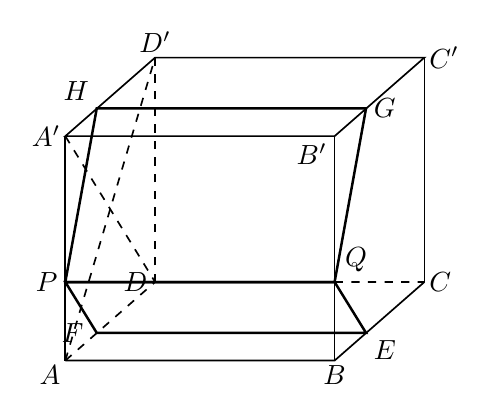
\begin{tikzpicture}[scale=0.95, semithick, every node/.style={inner sep=1.5pt}]
  \coordinate (A) at (0.00,0.00);
  \coordinate (B) at (3.60,0.00);
  \coordinate (C) at (4.80,1.05);
  \coordinate (D) at (1.20,1.05);
  \coordinate (A1) at (0.00,3.00);
  \coordinate (B1) at (3.60,3.00);
  \coordinate (C1) at (4.80,4.05);
  \coordinate (D1) at (1.20,4.05);

  \coordinate (P) at (0.00,1.05);
  \coordinate (Q) at (3.60,1.05);
  \coordinate (E) at (4.02,0.37);
  \coordinate (F) at (0.42,0.37);
  \coordinate (G) at (4.02,3.37);
  \coordinate (H) at (0.42,3.37);

  % 立方体可见棱
  \draw (A) -- (B) -- (C);
  \draw (A) -- (A1);
  \draw (B) -- (B1);
  \draw (C) -- (C1);
  \draw (A1) -- (B1) -- (C1) -- (D1) -- cycle;

  % 隐藏棱
  \draw[dashed] (A) -- (D) -- (C);
  \draw[dashed] (D) -- (D1);

  % 两个截面
  \draw[line width=0.9pt] (P) -- (Q) -- (E) -- (F) -- cycle;
  \draw[line width=0.9pt] (P) -- (Q) -- (G) -- (H) -- cycle;

  % 与截面平行的两条对角线
  \draw[dashed] (A1) -- (D);
  \draw[dashed] (A) -- (D1);

  \node[below left] at (A) {$A$};
  \node[below] at (B) {$B$};
  \node[right] at (C) {$C$};
  \node[left=1pt] at (D) {$D$};
  \node[left] at (A1) {$A'$};
  \node[below left=1pt] at (B1) {$B'$};
  \node[right] at (C1) {$C'$};
  \node[above] at (D1) {$D'$};
  \node[left=1pt] at (P) {$P$};
  \node[above right=2pt] at (Q) {$Q$};
  \node[below right=1pt] at (E) {$E$};
  \node[left=3pt] at (F) {$F$};
  \node[right=1pt] at (G) {$G$};
  \node[above left=1pt] at (H) {$H$};
\end{tikzpicture}
\end{center}
\nopagebreak[4]
\Needspace{4\baselineskip}
\textbf{解析}

（1）（2）同文科卷第 19 题：$\boldsymbol n_1=(0,1,1)$，$\boldsymbol n_2=(0,-1,1)$，$\boldsymbol n_1\perp\boldsymbol n_2$；$S_1=\sqrt2b$，$S_2=\sqrt2(1-b)$，和为 $\sqrt2$。

\Needspace{5\baselineskip}
（3）$D'(0,1,1)$，$E(1,b,0)$，$\overrightarrow{D'E}=(1,b-1,-1)$。由与平面 $PQEF$ 成 $45^\circ$：

\nopagebreak[4]
\[\frac{|b-2|}{\sqrt{2+(1-b)^2}\cdot\sqrt2}=\frac{\sqrt2}2\iff(1-b)^2+2(b-2)^2=4\left[2+(1-b)^2\right],\]

\Needspace{5\baselineskip}
化简得 $(1-b)^2=4$ 中取 $0<b<1$，解得 $b=\dfrac12$。此时

\nopagebreak[4]
\[\sin\theta=\frac{\left|\overrightarrow{D'E}\cdot\boldsymbol n_2\right|}{\left|\overrightarrow{D'E}\right|\left|\boldsymbol n_2\right|}=\frac{\left|-\frac12+1\right|}{\frac32\cdot\sqrt2}=\frac{\sqrt2}6.\]

\gkanswer{答案：（1）证明见解析；（2）定值 $\sqrt2$；（3）$\dfrac{\sqrt2}6$。}

\end{answer}
\begin{answer}
\gksolhead{20}{}

\textbf{题目}：

在直角坐标系 $xOy$ 中，点 $P$ 到两点 $(0,-\sqrt3)$，$(0,\sqrt3)$ 的距离之和为 $4$，设点 $P$ 的轨迹为 $C$，直线 $y=kx+1$ 与 $C$ 交于 $A$，$B$ 两点。

（1）写出 $C$ 的方程；

（2）若 $\overrightarrow{OA}\perp\overrightarrow{OB}$，求 $k$ 的值；

（3）若点 $A$ 在第一象限，证明：当 $k>0$ 时，恒有 $\left|\overrightarrow{OA}\right|>\left|\overrightarrow{OB}\right|$。

\Needspace{4\baselineskip}
\textbf{解析}

（1）$2a=4$，$c=\sqrt3$，$b=1$，焦点在 $y$ 轴上，故 $x^2+\dfrac{y^2}4=1$。

（2）代入得 $(4+k^2)x^2+2kx-3=0$，由 $\overrightarrow{OA}\perp\overrightarrow{OB}$ 得 $\dfrac{1-4k^2}{4+k^2}=0$，故 $k=\pm\dfrac12$。

\Needspace{5\baselineskip}
（3）设 $A(x_1,y_1)$，$B(x_2,y_2)$，$x_1+x_2=-\dfrac{2k}{4+k^2}$，$x_1x_2=-\dfrac3{4+k^2}<0$，故 $x_1$、$x_2$ 异号；$A$ 在第一象限且 $k>0$ 时 $x_1>x_2$。于是

\nopagebreak[4]
\[\left|\overrightarrow{OA}\right|^2-\left|\overrightarrow{OB}\right|^2=(1+k^2)(x_1^2-x_2^2)+2k(x_1-x_2)=(x_1-x_2)\cdot\frac{6k}{4+k^2}>0,\]

即 $\left|\overrightarrow{OA}\right|>\left|\overrightarrow{OB}\right|$。

\gkanswer{答案：（1）$x^2+\dfrac{y^2}4=1$；（2）$k=\pm\dfrac12$；（3）证明见解析。}

\end{answer}
\begin{answer}
\gksolhead{21}{}

\textbf{题目}：

在数列 $\{a_n\}$，$\{b_n\}$ 中，$a_1=2$，$b_1=4$，且 $a_n$，$b_n$，$a_{n+1}$ 成等差数列，$b_n$，$a_{n+1}$，$b_{n+1}$ 成等比数列。

（1）求 $a_2$，$a_3$，$a_4$ 及 $b_2$，$b_3$，$b_4$，由此猜测 $\{a_n\}$，$\{b_n\}$ 的通项公式，并证明你的结论；

（2）证明：$\dfrac1{a_1+b_1}+\dfrac1{a_2+b_2}+\cdots+\dfrac1{a_n+b_n}<\dfrac5{12}$。

\Needspace{4\baselineskip}
\textbf{解析}

（1）由 $2b_n=a_n+a_{n+1}$、$a_{n+1}^2=b_nb_{n+1}$ 依次求得上述各项，猜测 $a_n=n(n+1)$，$b_n=(n+1)^2$，代入两条件均成立，可用归纳法证明。

\Needspace{5\baselineskip}
（2）$a_k+b_k=k(k+1)+(k+1)^2=(k+1)(2k+1)$。首项 $\dfrac1{2\cdot3}=\dfrac16$；当 $k\geqslant2$ 时

\nopagebreak[4]
\[\frac1{(k+1)(2k+1)}<\frac1{2k(k+1)}=\frac12\left(\frac1k-\frac1{k+1}\right),\]

\Needspace{5\baselineskip}
故

\nopagebreak[4]
\[\sum_{k=1}^n\frac1{a_k+b_k}<\frac16+\frac12\left(\frac12-\frac1{n+1}\right)<\frac16+\frac14=\frac5{12}.\]

\gkanswer{答案：（1）$a_2=6$，$a_3=12$，$a_4=20$，$b_2=9$，$b_3=16$，$b_4=25$，$a_n=n(n+1)$，$b_n=(n+1)^2$；（2）证明见解析。}

\end{answer}
\begin{answer}
\gksolhead{22}{}

\textbf{题目}：

设函数 $f(x)=\dfrac{\ln x}{1+x}-\ln x+\ln(x+1)$。

（1）求 $f(x)$ 的单调区间和极值；

（2）是否存在实数 $a$，使得关于 $x$ 的不等式 $f(x)\geqslant a$ 的解集为 $(0,+\infty)$？若存在，求 $a$ 的取值范围；若不存在，试说明理由。

\Needspace{4\baselineskip}
\textbf{解析}

\Needspace{5\baselineskip}
（1）

\nopagebreak[4]
\[f(x)=\frac{\ln x}{1+x}-\ln x+\ln(x+1)=-\frac{x\ln x}{1+x}+\ln(x+1),\]

\nopagebreak[4]
\[f'(x)=-\frac{\ln x}{(1+x)^2}.\]

故 $f$ 在 $(0,1)$ 上递增、在 $(1,+\infty)$ 上递减，$x=1$ 处取极大值 $f(1)=\ln2$（也是最大值）。

（2）不存在。由（1）$f$ 在 $x=1$ 处取最大值 $\ln2$，且 $\lim\limits_{x\to0^+}f(x)=0$、$\lim\limits_{x\to+\infty}f(x)=-\infty$；对任意 $a$，$\{x\mid f(x)\geqslant a\}$ 都是有界区间（$a\leqslant\ln2$ 时为 $(0,x_a]$ 形状），不可能等于 $(0,+\infty)$。

\gkanswer{答案：（1）增区间 $(0,1)$，减区间 $(1,+\infty)$，极大值 $f(1)=\ln2$，无极小值；（2）不存在。}

\end{answer}